% Szkielet dla pracy inżynierskiej pisanej w języku angielskim.

\documentclass[english,bachelor,a4paper,oneside]{ppfcmthesis}

\usepackage[utf8]{inputenc}
\usepackage[OT4]{fontenc}
\usepackage{amsmath}
\DeclareMathOperator*{\argmax}{arg\,max}

% Authors here.
\author{%
   Katarzyna Zjawin \album{xxx} \and 
   Michał Nowicki \album{95883} \and 
   Olgierd Pilarczyk \album{xxx} \and 
   Jakub Wąsikowski \album{xxx}}
\authortitle{}                                        % Do not change.
\title{Biblioteka do rozpoznawania gestów dla kontrolera Leap Motion}        % Note how we protect the final title phrase from breaking
\ppsupervisor{dr~inż.~Wojciech Jaśkowski} % Your supervisor comes here.
\ppyear{2014}                                         % Year of final submission (not graduation!)

\begin{document}

% Front matter starts here
\frontmatter\pagestyle{empty}%
\maketitle\cleardoublepage%

% Blank info page for "karta dyplomowa"
\thispagestyle{empty}\vspace*{\fill}%
\begin{center}Tutaj przychodzi karta pracy dyplomowej;\\oryginał wstawiamy do wersji dla archiwum PP, w pozostałych kopiach wstawiamy ksero.\end{center}%
\vfill\cleardoublepage%

% Table of contents.
\pagenumbering{Roman}\pagestyle{ppfcmthesis}%
\tableofcontents* \cleardoublepage%

% Main content of your thesis starts here.
\mainmatter%



\chapter{Static gestures recognition}

As was already mentioned, the detected gestures can be divided into two groups: static gestures and dynamic gestures.
The static gestures can be understood as a chosen position and orientation of the fingers and hand in a single moment, while dynamic gestures are defined as a movement of the hand and fingers in time. 
The problem of recognition of those gestures is a subject of following chapter. 
Firstly, the proposed approach is presented, followed by the introduction to the evaluation scheme. 
In last section, the performed experiments are descriebed, which were used to examine the effectiveness of proposed static gesture recognition approach.

\section{Proposed methods}

The static gesture recognition problem can be stated as a problem invariant to time.
That means that for each detected hand, the position and orientation can be treated as a new data uncorrelated to previously classified data.
While this assumption means that one can easily generate multiple samples from the sensors in short time, it also gives an opportunity to look at the static gesture recognition problem as a problem of classification.

While for most 2D gesture recognition problems simple classification algorithms seems to work well enough, the 3D data is more complication to model by the set of features and finally successfully label.
While dealing with 3D data, the position and orientation of hand can be easily affected by the height of the hand above the sensor or small change in the orientation of the hand with respect to the sensor's coordinate system. 
It is intuitively understood, that the system should recognize those gestures as the one as they are similar.
To meet those requirement, one need to define what is meant by the ,,small'' change in orientation resulting in treating the static gestures as the same.

\begin{figure}[htb]
\centering
 \includegraphics[width=0.6\columnwidth]{figures/SVM.png}
 \caption[]{SVM is a technique searching for the hiperplane that maximizes the margin between classes\footnotemark}
 \label{svmmargin}
\end{figure}



To meet those requirements, the Support Vector Machines \cite{Cortes:SVM} were used as a classification algorithm.
The SVMs were chosen as there exist a solid mathematical background supporting the simple idea of maximalizing the margin between classes.
Moreover, the SVMs were chosen also because of the popularity due to the open-source library libSVM \cite{libSVM}, which contains the multiple platform SVM implementation.
It is worth noticing that in original work, SVMs were used only to classify between two classes, but the idea was expanded to utilize the one-vs-all scheme allowing to classify multiple class sets.
The efficiency of SVMs depends on correctly choosing the kernel function used to map the separation problem into higher-dimension with expectation to achieve problem easier to solve.
The typical kernel functions:
\begin{itemize}
\item linear: $K(x_i, x_j) = x_i^Tx_j$.
\item polynomial: $K(x_i, x_j) = (\gamma x_i^Tx_j + r)^d, \gamma > 0$.
\item radial basis function (RBF): $K(x_i, x_j) = exp(-\gamma ||x_i - x_j||^2), \gamma > 0$.
\item sigmoid: $K(x_i, x_j) = tanh(\gamma x_i^Tx_j+r)$.
\end{itemize}
where $\gamma$, $r$, and $d$ are kernel parameters. According to the authors of the library, linear kernels should be used for linearly separable problems, while RBF kernel is the most versatile one.

\footnotetext{\url{http://en.wikipedia.org/wiki/File:Svm_max_sep_hyperplane_with_margin.png}}

The problem of classification assumes that each sample consists of set of features, which describe this sample and can be used to distinguish it from the other samples.
Additionally, each sample has a known or unknown label, which defined the membership of sample to the class. 
The samples with the known labels can be used to train the classification system to compute the membership to the classes for the samples. 
The computation is performed on previously mentioned sets of features.

In application of gesture recognition the classification be divided into two flows: the training part and the recognition part. 
In training part, the library will be provided with the samples of static gestures with known correspondences to the static gesture classes. 
From those samples, the sets of features are computed, which are used to train the classifier.
The recognition part assumes to have trained classifier. 
The recognition part is provided with samples static gestures without labels. 
For each sample the sets of features are computed and then given as input to the trained classifier.
The classifier returns the information of the gesture's class membership (label) of each sample.

In case of library, it is assumed that the learning process can be done offline, while strict online requirements has to be met in recognition part. 
To meet those requirements the Support Vector Machine is introduced[]. 
The SVM classification is commonly used technique in multiple areas of research as biology, robotics or IT for solving data classification problems [].
Additional advantage of the SVM is possibility to use C++ library libSVM[], which provides an easy interface to utilize this classification methods in different problems.

\begin{figure}[htb]
\centering
 \includegraphics[width=1\columnwidth]{figures/StaticGestures.png}
 \caption[]{Proposed solution blocks for learning and recognitnion parts of static gestures recognition problem}
 \label{svmmargin}
\end{figure}


While presented approach can be treated as state-of-the-art approach it still cannot be used without defining proper feature sets for gesture recognition.
The naive solution would be to use the raw data from Leap motion sensor as the feature set.
This solution was tested, but provided poor results as the proposed features were dependent on the position, orientation and scale of hand. 
Even small movement in any direction meant problems with stable recognition. 
The theoretical literature suggests to compute a set of features invariant to wanted transformations, which can allow to fully distinguish between different classes.
Unfortunately, there are not available propositions to feature sets when it comes to the gesture recognition using the data even similar to the data provided by the Leap Motion sensor.
Reminding, the Leap Motion for each frame allows to capture:

\begin{itemize}
\item position in X, Y, Z of each recognized finger
\item unit vector of each recognized finger
\item the width and height of each finger
\item the normal vector of the hand
\end{itemize}


\section{Evaluation methodology}

\subsection{Assumptions}
To provide user with library working in different conditions, it was assumed that the gesture is treated as the same one independently with respect to the translation, rotation and scale of the hand. 
This assumption means that the static gesture rotated by unknown angles, translated in sensor coordinate system and also with different hand sizes should still be recognized as the same gesture.
Invariance to the rotation, translation and scale poses a great challenge to the recognition, but allows the future users of API to fully utilize the feasibility of the library.
It is worth mentioning that, it does not reduce the possible applications of the library, as an assignment of static gesture to already defined class allows to find the transformation between the model of the class and observed gesture.


\section{Recorded datasets}

To propose and test the quality of the features twelve static gestures were chosen:
\begin{enumerate}
\item the peace sign,
\item a fist,
\item full hand with space between each finger,
\item American Sign Language: ``I love you'' sign,
\item sign ``gun'' created by putting thumb and forefinger up, while holding the rest fingers in a fist,
\item all fingers in a fist with exception of thumb, which is up,
\item the sign X made with the forefingers of both hands,
\item the sing ``Time'' used e.g. by coaches in basketball games.
\item sign simulating rotating a knob by two fingers,
\item sign simulating rotating a knob by five fingers.
\end{enumerate} 
The gestures are also presented at fig.~\ref{staticgestures}.

\begin{figure}[htb]
\centering
 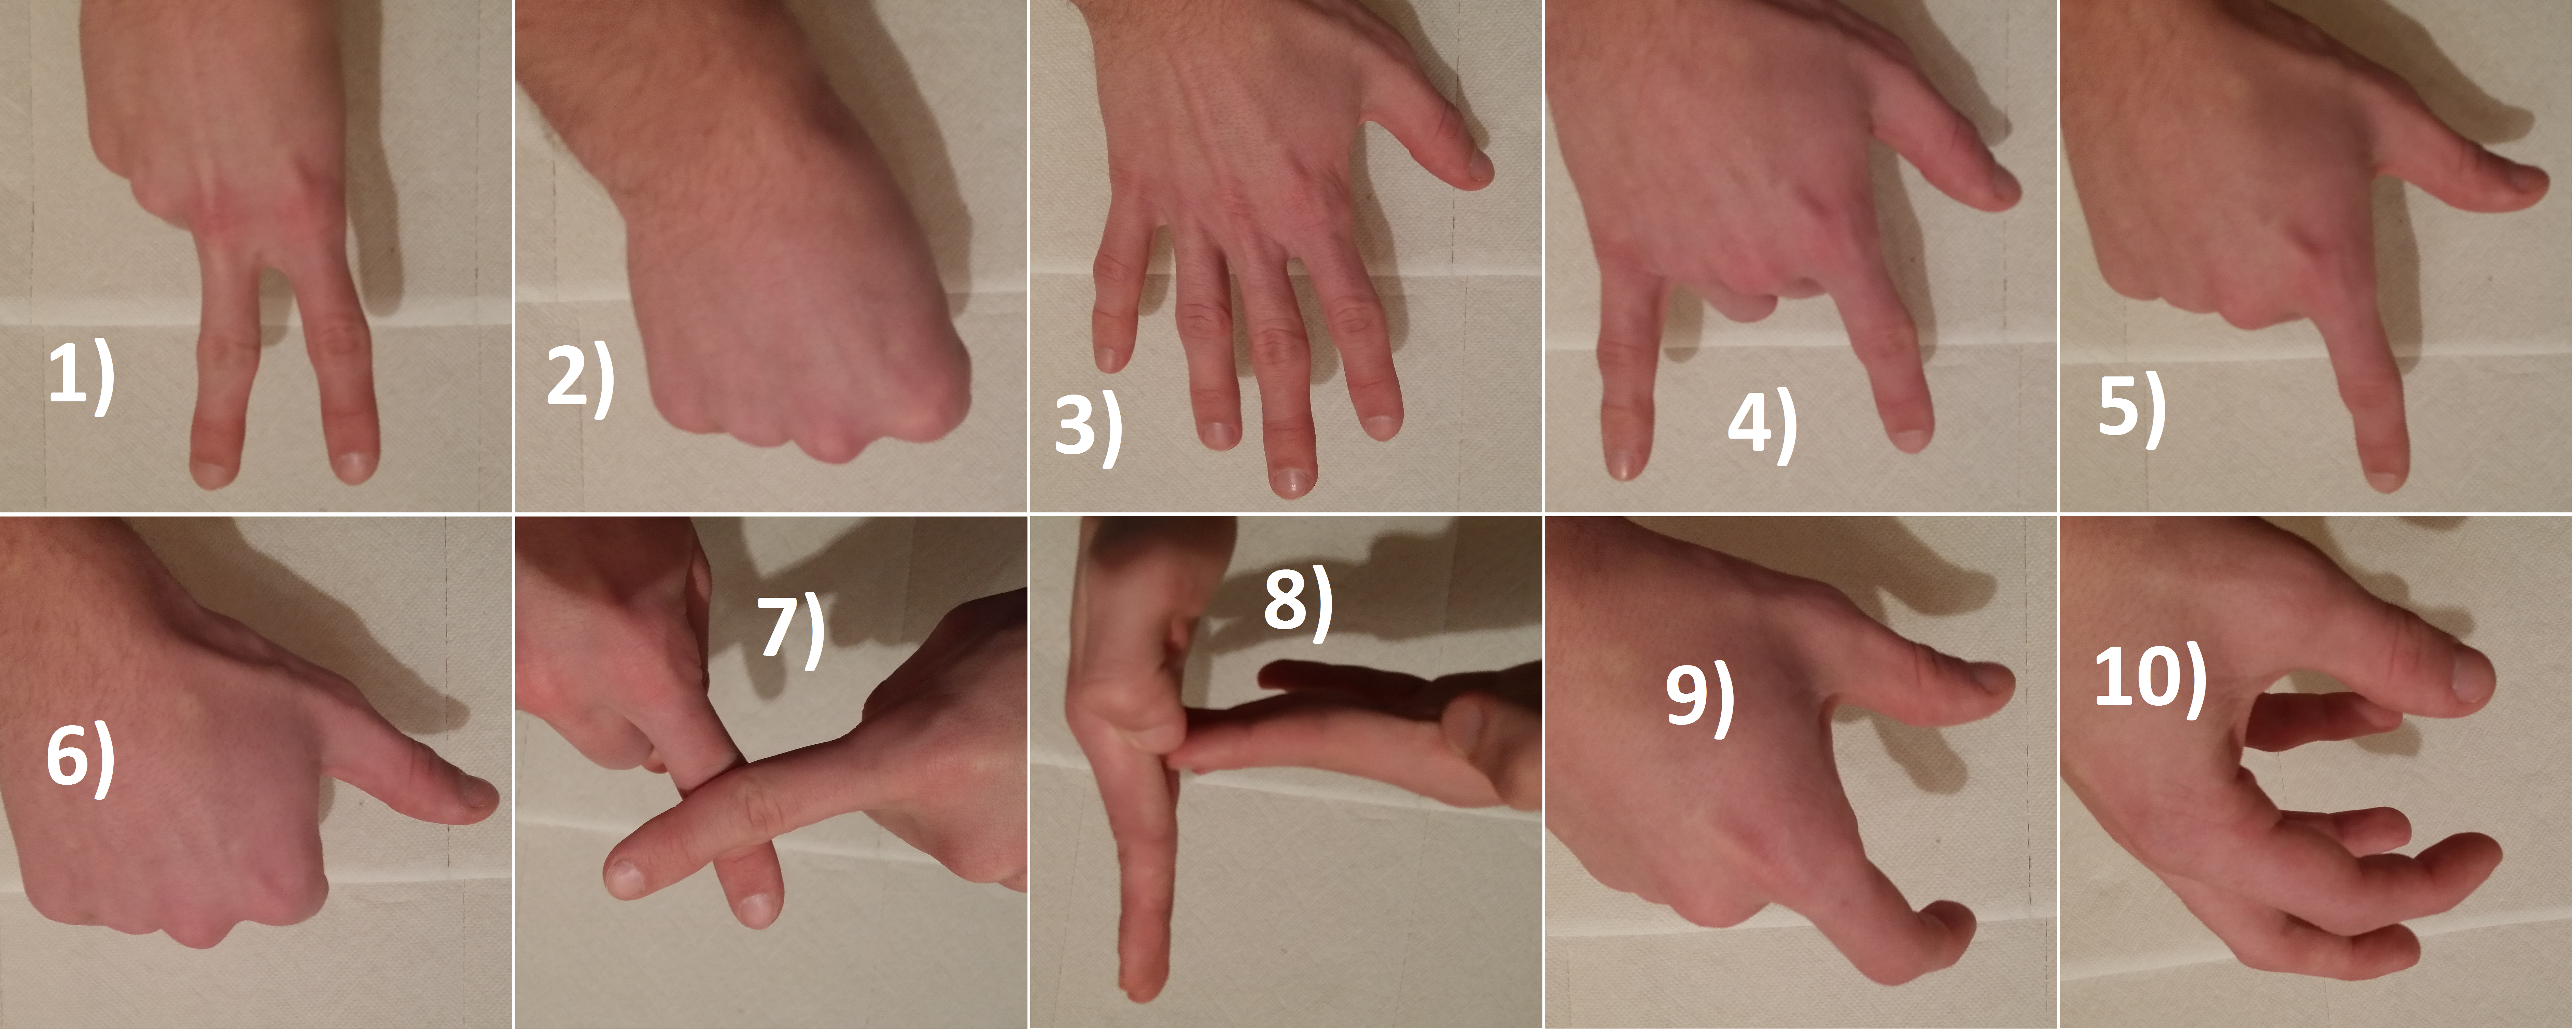
\includegraphics[width=1.0\columnwidth]{figures/static_gestures.png}
 \caption{Figures chosen for the comparison of different classification approaches}
 \label{staticgestures}
\end{figure}

The sample data of each gestures were recorded using the continuous mode of recording, while moving the hands in different directions and changing the orientation of the hands. 
For each of the proposed gestures, each author recorded approximately 1000 samples.

Having samples with known labels, the whole dataset was separated into training and testing sets in relation 2:1. 
For the training, the k-fold cross-validation (CV) scheme was used, which searches for optimal $C$ and $\gamma$ parameters trying to prevent the algorithm from over-fitting the training data.
This method is used to find the optimal parameters of the classification system, while estimating the performance on the data not used in the training part. 
In standard version of the method, the gathered data is divided into two sets: one containing k-1 parts of the data, the other 1 part of the data. 
The first is used to train the classification system, while the rest of the gathered data is used to estimate the performance. 
The performance is estimated by calculating the number of cases when the classification system returned a label which matched already known label. 
The percent of correctly recognized labels to the total size of the testing set is known as recognition rate.



The first proposed vector of features consisted of:
\begin{itemize}
\item number of fingers in frame,
\item the absolute angles between fingers and the normal of the hand,
\item the absolute angles between consecutive fingers,
\item the euclidean distance between consecutive finger's tips.
\end{itemize} 

After approach allowed to achieve XXX\% of recognition rate and was unsatisfying from the perspective of feature application. 
Analysis of the finger numbering revealed that the fingers are numbered accordingly to the position in Z axis of the tip of the finger.
This means that when features are approximately on the same position in Z axis, the numbering can change rapidly and proposed features compare different fingers.
To achieve the features that would be invariant to the numbering of the fingers, the feature set was changed.
Instead of containing the absolute angles and distances between consecutive fingers, it was proposed to contain the five greatest values of angles and five greatest values of distances between all combinations of finger pairings.
This approach was tested on the same training set and allowed to increase the recognition rate to the 83.8812\%.
While the number of fingers in frame and five greatest angles between all possible angles between fingers are invariant to the translation, rotation and scale, the distances between tip position were dependent on the scale of hand.
To achieve distances invariant to the scale of hand, it was proposed to exchange the five greatest distances for five greatest ratios of the distances between tips of all fingers to the maximal found distance between tips of all fingers.
As this approach was expected to increase the recognition rate, it fell down to 77.0913\%.
More experiments with enlarging the set of features to having ten greatest angles and ten greatest distances showed slight fall in recognition rate to 83.7687\%. 
The all results have been presented in table [].

To increase the recognition rate an attempt to gather more training data was performed, which end with recognition rate equal to XX\%. 
While using more data, it is worth noticing the growth of training time. In case of 5000 samples the typical training process took approximately 6 hours. 
This computing time can be unacceptable by the users of the library, so the test with another SVM library libLinear[] was performed. 
The libLinear's implementation of SVM utilizes the linear kernels, which are useful for large data training sets with multiple number of features. 
This library reduced the training time to about 20 seconds, but the best obtained recognition rate was 64.524\% for libLinear compared to the 83.8812\% for the libSVM.


The firstly tested set of static gestures contained gestures, which were did not take into account the way how the Leap Motion works and for gestures like fist or 'X' the recorded data contained almost no information how to classify those gestures.
That's why the experiments were repeated on the five gestures, which could be easily distinguishable by data provided by Leap Motion. To this experiment the gestures peace, hand, ''I love you'', fist with thump up and rotating knob by 5 fingers were chosen.
For this classification problem with feature set defined by number of fingers, 5 greatest absolute angles and 5 greatest absolute distances between fingers, the recognition rate of 90.9532\% was achieved. 

The last test performed for static gestures recognition consisted of classifying the set of 10 possible static gestures. For this test the recognition rate of 73.2118\% was achieved.


\chapter{Detection of dynamic gestures}

\section{Proposed methods}

The dynamic gesture recognition problem is a problem, where the input data consist of several consecutive positions and orientations of hand and fingers. 
Moreover, the important factor for recognition is the time dependencies between data frames. 
The slower and faster gestures should be recognized as the same dynamic gesture.

The proposed solution utilizes parts of the solution used for recognition of the static gestures.
Each frame of the captured data is described by the same features as in the static recognition part.
The set of features for each frame is then processed by the Hidden Markov Model scheme. 

\subsection{Hidden Markov Model}

Hidde Markov Model is a finite, $N$-element set of states, which are associated with the probability distribution.
The transitions between states are represented by the transition probabilities usually stored in $N\times N$ matrix $T$.
In every state, one of the observation from the finite, $K$-element observation set can be generated with observation probability usually represented by the $N\times K$ emission matrix $E$.
The finite set of all possible observation is called the alphabet.
To fully define the model, the definition of $N$-element vector of initial state probabilities $\Pi$.
Each HMM can be fully defined by the ($T$, $E$, $Pi$).

\begin{figure}[htb]
\centering
 \includegraphics[width=0.8\columnwidth]{figures/HMM_wiki.png}
 \caption[]{Solution blocks of learning and testing parts in task of dynamic gesture recognition\footnotemark}
 \label{dynamicgestureswiki}
\end{figure}

\footnotetext{\url{http://en.wikipedia.org/wiki/File:HiddenMarkovModel.svg}}

The example HMM can be seen at fig.~\ref{dynamicgesturewiki}.
The HMM at the figure consists of 3 states ${X1, X2, X3}$ and 4 possible observations ${y1, y2, y3, y3}$.
The probabilities $a_{ij}$ define the transition probability from state $j$-th to state $i$-th. 
The probabilities $b_{ij}$ define the observation probability of generating $j$ observation while being in state $i$.

The HMM can be understood as a directed graph with two types of weighted vertices. 
This way, each state is represented by one type of vertices while observations can be shown as second type of vertices.
The edges between states contain and are an equivalent to the transition matrix. 
There are no edges between vertices representing observations.
The edges between states and observations are equal to the observation matrix.

$ xx $
There are three main algorithms used with the HMMs:
\begin{itemize}
\item Forward-Backward algorithm, 
\item Viterbi algorithm,
\item Baum-Welch algorithm.
\end{itemize}

The Forward-Backward algorithm is used to find the posterior probability of given states given the set of observations.
For the whole set of state variables $X = {X_i}_{i=1}^{N}$ and a set of observations $o_{1:t} = o_1, o_2,...,o_t$, the algorithm computes the $P(X_i | o_{1:t})$.
The algorithm utilizes a dynamic programming approach, by perfoming 3 steps in a loop: 
\begin{enumerate}
\item computing forward probabilities,
\item computing backward probabilites,
\item computing smoothed values.
\end{enumerate}
Firstly, the forward pass phase for $i=1,..,N$ computes the $P(X_i, o_{1:k})$, where $k$ is smaller than $t$, which represent the probability of ending up in state $X_i$ after first $k$ observations. 
The backward pass computes the $(P(o_{k+1:t}) | X_i)$, which are the probabilities of observing the rest of the observations in state $X_i$.
The smooting part, uses Bayes rule to compute the probability of state $X_i$ given the whole observation sequence:
\begin{equation}
P(X_k | o_{1:t}) = P(X_k | o_{1:k}, o_{k+1:t}) \propto P(o_{k+1:t} | X_k) P(X_k | o_{1:k})
\end{equation}
The time complexity of this algorithm is $O(N^2 T)$, where $T$ is the length of observation sequence and $N$ is the number of possible states.

The Viterbi algorithm is used to find the most likely sequence of hidden states that best explain the set of observations.
The set of those states is usually called the Viterbi path. 
Introduing the sequence:
\begin{equation}
V_{1,k} = P(o_1 | k) * \Pi_k)
\end{equation}
\begin{equation}
V_{t,k} = P(o_t | k) * argmax_{x\in X}(a_{x,k} * V_{t-1,x})
\end{equation}
Finally, the problem can be understood as finding the $argmax_{x\in X}(V_{T,x})$. 
The algorithm time complexity is the same as forward-backward $O(N^2 T)$.

The Baum-Welch algorithm is the algorithm used to find the unknown parameters of the HMM.
For each training example, the algorithms updates the state transition probabilities, observation probabilities in each state and intial probabilities to maximize the likelihood of observation.
Having the set of sets of observations, the algorithm can be used to train HMM to detect the sequences similiar to the ones used in learning process.

\begin{figure}[htb]
\centering
 \includegraphics[width=1\columnwidth]{figures/SingleHMM.png}
 \caption{Non-zero state transitions and states of the HMM used to detect single dynamic gesture}
 \label{singlehmm}
\end{figure}

In the dynamic gesture recognition task, we adopted a structure of HMM with state having non-zero transition probabilites to self and to the next state in the sequence.
The proposed structe is presented at fig.~\ref{singlehmm} 
The states can be understood as the phases of hand movement and position that happen when the wanted gesture is performed.
The self-transitions are used to model the different speeds of the gestures.
This structure after training process can be used to measure the probability of that the dynamic gesture occured given the set of observations.

\begin{figure}[htb]
\centering
 \includegraphics[width=1\columnwidth]{figures/HMM_eng.png}
 \caption{Non-zero state transitions and states for the HMM enabling simulatneous detection of $m$ dynamic gestures}
 \label{HMMstructure}
\end{figure}

Having single dynamic gesture recognition problem modelled as the sequence of $n$ states in which $kths$ state is connected by the edges to the $k$ and $(k+1)$ state and to the all observations.
Having the problem of distinguishing $m$ gestures translates to the $m$ sequential graphs.
The problem of finding if and what dyanmic gesture occured is the problem of finding the probabilities from each $m$ HMM and checking them against preset threshold.
Alternatively, the $m$ HMMs can be combined into one HMM were those single HMMs are treated as parallel paths.
The structure of proposed single HMM is presented at fig.~\ref{HMMstructure}.
Then the recognitnion process is a process of finding, which of the parallel paths is the most probable.
The only remaining problem is the problem of preparing the set of ccured, 1-dimensional observations from the Leap Motion data.

\subsection{HMM observation from Leap Motion data}

Most of the proposed solutions in the literature assume that the observations are 1-dimensional.
There were attempts to expand the HMM to the 2-dimensional observations [], but the raw data from Leap Motion is defined in higer-dimensional that any found solution.
That is the reason, why the need to reduce the dimensionality of the observation of the single hand in the predefined moment in time.

To do this, unsupervised clustering algorithms were used.

***********************
**************8
Opisać algorytmy
Opisać metody doboru liczby klas
********


\begin{figure}[htb]
\centering
 \includegraphics[width=1\columnwidth]{figures/DynamicGestures.png}
 \caption{Solution blocks of learning and testing parts in task of dynamic gesture recognition}
 \label{dynamicgesturesflow}
\end{figure}

Finally, the whole processing flow has been desgined and is presented at fig.~\ref{dynamicgesturesflow}.
The whole solution consists of two parts: offline learning and online recognition.
For learning, the raw data is preprocessed and then the feature are extracted. 
Similarly to the static gestures, the features set containing the finger count, angles between fingers and normal of hand, angles between fingers and distances between finger's tips were used. 
In traning part, those features are extracted from all recorded positions for all dynamic gestures.
Then one of the unsupervised clustering algorithms is used to find the classes of observations (usually 8-12 classes worked best).
Knowledge of the classes is used to represent each dynamic gesture as a series of one-dimensional observations.
After that for each dynamic gesture, the corresponding HMM is learned by running the Baum-Welch algorithm on the sequence of observations.
To complete, the training process, the HMMs are combined into one HMM.

In the online working, the raw data from leap motion is preprocessed, then each frame is labeled accordingly to the classes learnt by the unsupervised clustering algorithm.
The next step include providing the set of observations to HMM and running the Viterbi algorithm.
The Viterbi algorithm finds the most likely sequence in one the parallel paths, which informs us about the number of the found gesture. 
If the likelihood is above preset threshold, the gesture is assumed to be correctly recognized.


\section{Evaluation methodology}

To evaluate proposed approach ... 






  






The proposed solution utilizes Hidden Markov Model[] 



\section{Experiments}


% All appendices and extra material, if you have any.
\cleardoublepage\appendix%
%\input{0a-appendix.tex}

% Bibliography (books, articles) starts here.
\bibliographystyle{alpha}{\raggedright\sloppy\small\bibliography{bibliography}}

% Colophon is a place where you should let others know about copyrights etc.
\ppcolophon

\end{document}
